\subsection{Linkages}
%graph -> G = (V,E)
%linkage -> (G,l)
%embedding -> 
There are two parts to a linkage, the graph and the edge length mapping, e.g. $(G,l)$.  While 
graphs can have 
vertices that may not correspond to any edges, we rule out 
this possibility for linkages.  Like a graph, a linkage is still an abstract combinatorial 
structure until an \textit{embedding} on the 
graph of the linkage is posed and the definitions of a proper embedding and realization of a  graph 
are the same for embeddings.  
%needs to explain edge crossings, loops, and multiedges.
\subsubsection{Edge Crossings}
\begin{figure}[H]
\begin{center}
    %add desired spacing between images, e. g. ~, \quad, \qquad etc.
    %(or a blank line to force the subfigure onto a new line)
  \begin{subfigure}[b]{0.24\textwidth}
	  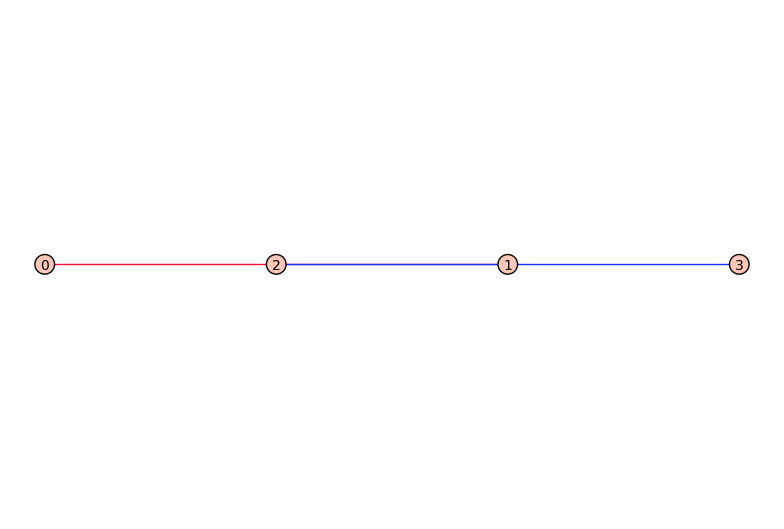
\includegraphics[width=\textwidth]{graphics/crossingType1.png}
	  \caption{An edge crossing where two edges overlap.}
	  \label{fig:ch1-linkages-1-1}
  \end{subfigure}
  \begin{subfigure}[b]{0.24\textwidth}
	  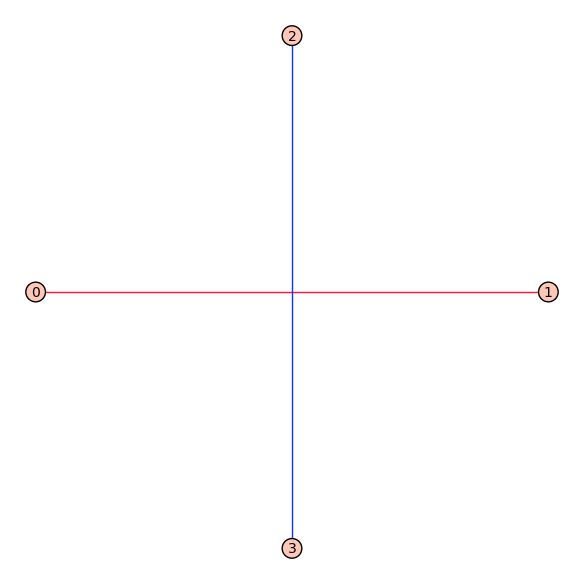
\includegraphics[width=\textwidth]{graphics/crossingType2.png}
	  \caption{An edge crossing where two edges intersect at a point.}
	  \label{fig:ch1-linkages-1-2}
  \end{subfigure}
  \begin{subfigure}[b]{0.24\textwidth}
	  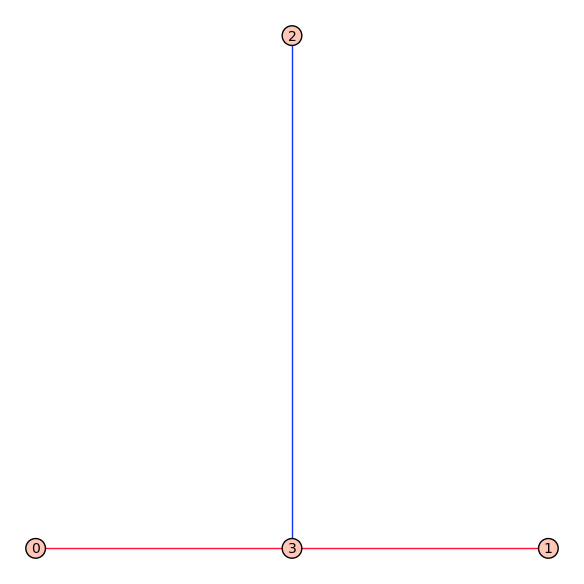
\includegraphics[width=\textwidth]{graphics/crossingType3.png}
	  \caption{An edge crossing where two edges intersect at a vertex.}
	  \label{fig:ch1-linkages-1-3}
  \end{subfigure}
  \begin{subfigure}[b]{0.24\textwidth}
	  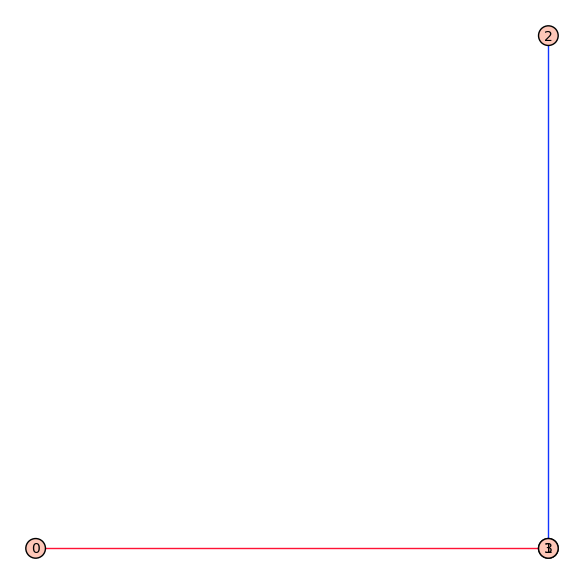
\includegraphics[width=\textwidth]{graphics/crossingType4.png}
	  \caption{An edge crossing where two edges intersect at two vertices.}
	  \label{fig:ch1-linkages-1-4}
  \end{subfigure}
\end{center} 
\caption{These figures exhibit the 4 types of edge crossings.}\label{fig:ch1-linkages-1}
\end{figure}
\subsubsection{Loops}
\subsubsection{Multi-edges}
Without loss of generality, for this paper, we focus on 
linkages that have simple planar graph properties, i.e.:
\begin{itemize}
\item[\rn{1}] does not have edges that cross,
\item[\rn{2}] does not have loops, i.e. $(v,v) \in E$, or
\item[\rn{3}] does not have multiple edges between any pair of vertices.
\end{itemize}  
We may visit special cases in which we look at planar graphs that satisfy the last two conditions 
but not the first, e.g.:
%graph component of the linkage   the plane.  A linkage 
%\textit{embedding} is $L : V \mapsto 
%\bbR^{2}$.
% A \textit{linkage} is an ordered pair $G = (V,E)$ comprising of a set $V$ of vertices or nodes 
% together with a set $E$ of edges or lines. This definition is commonly used for graphs.  Mapping 
% the linkage $G$ into the plane is said to be the \textit{embedding}, i.e. $L : V \mapsto 
% \bbR^{2}$.  A length function correspond to a linkage, $l: E \mapsto \bbr^+$ gives a length to an 
% edge in the linkage.  If We consider a \textit{realization} of a linkage is range of $L$, i.e. 
% $L(V)$. If for every edge $(u,v) \in E$ such that $l\left( \left(u,v\right) \right) = \left\vert 
% L(u) - L(v) \right\vert$ is true, then $L$ is said to be a \textit{proper embedding} of $G$.
\begin{figure}[h]
\begin{center}
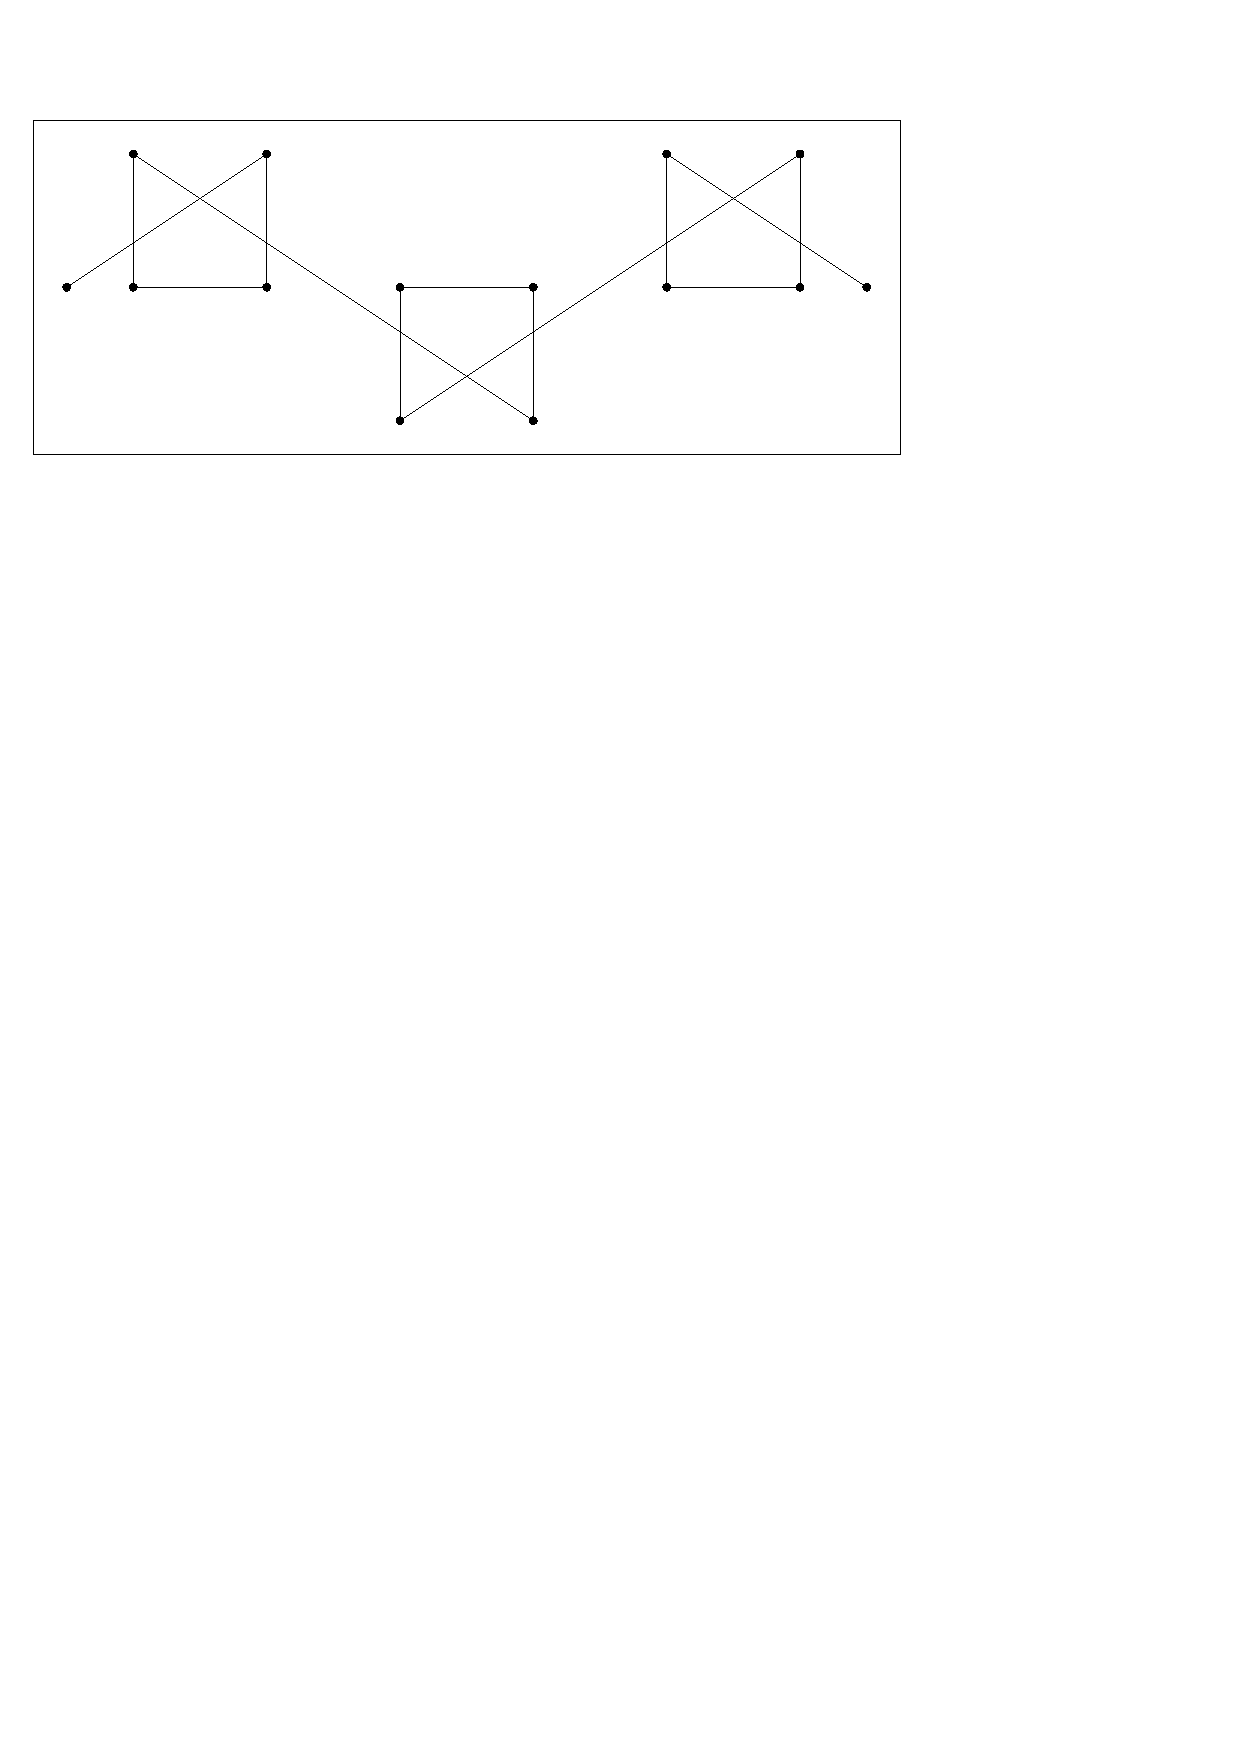
\includegraphics[scale=1]{graphics/crossingEdgeLinkage.pdf}
\end{center} 
\caption{A linkage where edges cross however it does not contain loops or multiple edges between 
vertices.}
\label{fig:linkage-3}
\end{figure}
